    \subsection{Performance Analysis}
    \label{subsec:performance-analysis}

    This subsection presents the experimental evaluation of VeRedact-PQ
    under increasing redaction workloads, committee configurations, audit
    scopes, and on-chain anchoring costs. The objective is to assess whether
    the proposed batching, coalescing, and cost-aware auditing mechanisms
    improve end-to-end redaction efficiency while preserving the
    request-level validation and post-quantum protection defined in
    Section~\ref{sec:security}.

    \subsubsection{Experimental Setup}

    \chg{VeRedact-PQ and the four baselines~\cite{ref1,ref13,ref27,ref34} were
    implemented in approximately 9{,}300 lines of Python, Rust, and Solidity
    code and evaluated on an AWS c7i.4xlarge server with an Intel Xeon
    Platinum 8488C processor (16 vCPUs) and 32\,GB RAM, running Ubuntu 24.04.
    The Besu validator nodes ran as Docker containers on this host, and
    inter-node latency was set to 10\,ms using Linux \texttt{tc netem} to
    emulate a multi-organization deployment; committee members, the VPS, the
    audit service, and the auditor ran as processes on the same host. In
    Experiment~1, requesters generated their signatures and PQZK proofs on
    two separate c7i.48xlarge hosts, so that requester-side proving did not
    consume the cores of the system under test.}

    PQSIG was instantiated with ML-DSA-65 (FIPS~204) through the Open Quantum
    Safe \texttt{liboqs} library. $H$, $H_1$, $H_2$, and $H_A$ were
    instantiated as domain-separated SHA3-256, and $\mathsf{PRF}$ as
    HMAC-SHA3-256 with 256-bit keys $K_{\mathrm{idx}}$
    and $K_A$ { ($\lambda=256$)}, consistent with the {$\lambda$}-bit key length of Phase~1. PQZK was instantiated with a transparent hash-based
    STARK proof system \chg{(winterfell~0.13; 42 queries, blowup factor~8,
    16-bit grinding)}, consistent with the
    trapdoor-free setup assumed in Phase~1. PQCH was implemented as an
    SIS-based chameleon hash following~\cite{ref10,ref17}, with distributed
    adaptation realized through $t$-of-$n$ trapdoor sharing
    \chg{of a gadget-based lattice trapdoor, dealt without a trusted dealer}. Merkle structures, BIMC, SA-RLI,
    and RAI use binary SHA3-256 trees with multiproof support. The PBN was
    deployed as a \chg{7}-validator Hyperledger Besu network using
    QBFT consensus \chg{with a 2-s block period}, with Solidity contracts anchoring policy commitments,
    committee configurations, batch checkpoints, and RAI checkpoints; PQ
    signature verification is performed by the validator nodes before
    anchoring rather than inside the contracts. Table~\ref{tab:primitives}
    reports the measured execution time of each primitive.

    The workload consists of synthetic enterprise transactions with payloads
    of 256\,B to 4\,KB, organized into transaction batches of $N$ leaves.
    Redaction targets follow a Zipf distribution with skew $s$ to control
    batch locality, where $s=0$ corresponds to uniformly distributed targets
    and larger $s$ concentrates requests on fewer transaction batches.
    Request arrivals follow a Poisson process whose rate is varied per
    experiment\chg{, and every scheme replays the same request trace generated
    from one seed}.
    Unless otherwise stated, the parameters in Table~\ref{tab:params} are
    used\chg{. Each configuration point is executed once; reported values are
    medians (95th percentiles for latency) over all requests or samples of
    that run, and primitive timings are medians with 95\% confidence
    intervals.}

    To separate architectural effects from primitive choice, all baselines were reimplemented within the same framework and
    instantiated with their own classical primitives at about 128-bit
    security, since none of their papers defines a post-quantum variant.
    Stages not
    defined by a baseline's paper are reported as not supported. Each baseline otherwise follows its original
    workflow, including per-request authorization and adaptation.
    \chg{For auditing, Scheme~\cite{ref1} holds its accumulator membership
    proofs locally, an option its paper provides, and the per-record
    accumulator witnesses of Scheme~\cite{ref13} are timed individually on one
    core and summed. The redaction histories audited in Experiments~3 and~4
    are built beforehand and are not timed.}

    \begin{table}[t]
    \centering
    \caption{Execution Time of Cryptographic Primitives}
    \label{tab:primitives}
    \scriptsize
    \renewcommand{\arraystretch}{1.08}
    \setlength{\tabcolsep}{4pt}
    \begin{tabular}{llc}
    \hline
    \textbf{Operation} & \textbf{Instantiation} & \textbf{Time (ms)} \\
    \hline
    \multicolumn{3}{l}{\textit{VeRedact-PQ}} \\
    $T_S$ / $T_V$ & ML-DSA-65 sign / verify & \chg{0.078 / 0.031} \\
    $T_{ZP}$ / $T_{ZV}$ & PQZK prove / verify & \chg{20.689 / 0.647} \\
    $T_{CH}$ & PQCH hash & \chg{1.087} \\
    $T_{PA}$ / $T_{CB}$ & PQCH partial adapt / combine & \chg{21.992 / 6.247} \\
    $T_H$ & SHA3-256 (64-byte input) & \chg{0.001} \\
    $T_{\mathrm{PRF}}$ & HMAC-SHA3-256 & \chg{0.004} \\
    \hline
    \multicolumn{3}{l}{\textit{Baselines}} \\
    $T_V^{c}$ & ECDSA secp256k1 verify~\cite{ref1,ref27} & \chg{0.047 / 0.025} \\
    $T_{PA}^{c}$ / $T_{CV}^{c}$ & Improved DCH, BLS12-381~\cite{ref1} & \chg{1.144 / 2.372} \\
    $T_{PA}^{c}$ / $T_{CV}^{c}$ & ETCH, secp256k1~\cite{ref27} & \chg{0.036 / 0.053} \\
    $T_{AD}^{c}$ / $T_{CV}^{c}$ & Double-trapdoor CH, RSA-3072~\cite{ref13} & \chg{7.520 / 8.059} \\
    $T_{AD}^{c}$ / $T_{CV}^{c}$ & CHET, RSA-3072~\cite{ref34} & \chg{53.527 / 47.661} \\
    $T_{Acc}$ & RSA-3072 accumulator~\cite{ref1,ref13} & \chg{0.652} \\
    $T_{Tag}$ & Identity-based RSA-3072 tag~\cite{ref13} & \chg{58.816 / 51.813} \\
    $T_{Pol}$ & MA-ABE decryption, BLS12-381~\cite{ref34} & \chg{7.269} \\
    \chg{$T_E^{c}$} & \chg{RSA-3072 exponentiation~\cite{ref13}} & \chg{7.334} \\
    \hline
    \end{tabular}
    \end{table}

    \begin{table}[t]
    \centering
    \caption{Default Experimental Parameters}
    \label{tab:params}
    \scriptsize
    \renewcommand{\arraystretch}{1.08}
    \setlength{\tabcolsep}{4pt}
    \begin{tabular}{ll}
    \hline
    \textbf{Parameter} & \textbf{Default value} \\
    \hline
    Committee size $n$ / threshold $t$ & [7] / [5] \\
    ABRRR bounds $B_{\min}$ / $B_{\max}$ & [8] / [256] \\
    Maximum waiting time $T_{\max}$ & [500]\,ms \\
    Transaction leaves per batch $N$ & [256] \\
    SA-RLI shards $S$ / RAI shards $S_A$ & [16] / [16] \\
    Ledger size & [$10^5$] transactions \\
    Zipf skew $s$ & [0.8] \\
    Signature scheme & ML-DSA-65 (NIST category 3) \\
    \chg{Runs} & \chg{1 per point; 30 samples per point (Exp.~2--4)} \\
    \hline
    \end{tabular}
    \end{table}

    % ---------------------------------------------------------------------
    \subsubsection*{\textbf{Experiment 1: Redaction Latency and Throughput}}

    This experiment evaluates end-to-end redaction performance \chg{as the
    request arrival rate increases from 100 to 5{,}000 requests/s} over the
    default ledger, \chg{comparing VeRedact-PQ with Refs.~\cite{ref1},
    \cite{ref13}, \cite{ref27}, and~\cite{ref34}}. End-to-end latency is
    measured from request submission to blockchain finalization of the
    updated checkpoint, covering Phases~3 to~5, and throughput is measured as
    \chg{the number of redactions finalized per second within a 60-s window
    that follows a 10-s warm-up}. To evaluate the effect of batch locality,
    the Zipf skew is additionally varied as $s\in\{0,0.4,0.8,1.2\}$ at
    \chg{100 requests/s}, and the number of distributed PQCH adaptations per
    1,000 finalized redactions is recorded. The results are shown in
    Fig.~\ref{fig:exp1_redaction}.

    \begin{figure}[t]
    \centering
    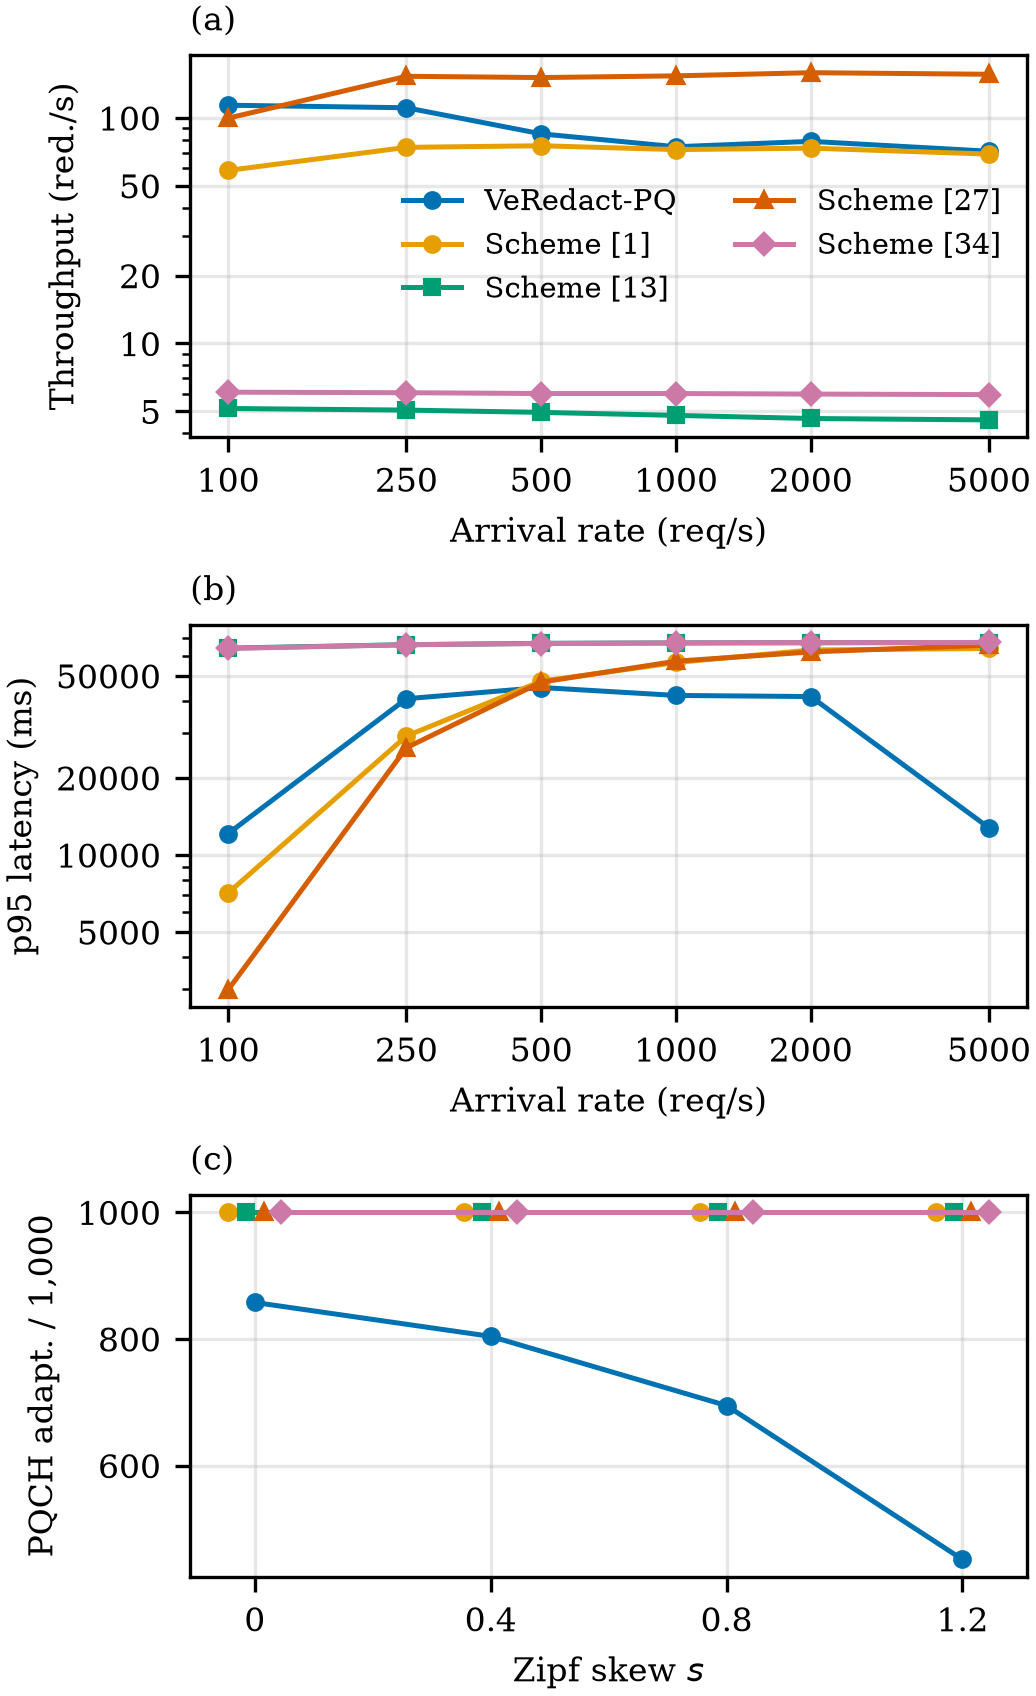
\includegraphics[width=0.8\linewidth]{exp1_redaction_throughput.png}
    \caption{Redaction performance: (a) throughput and
    (b) 95th-percentile end-to-end latency versus request arrival rate, and
    (c) PQCH adaptations per 1,000 redactions versus Zipf skew.}
    \label{fig:exp1_redaction}
    \end{figure}

    \chg{Fig.~\ref{fig:exp1_redaction}(a) shows that Ref.~\cite{ref27}
    achieves the highest throughput, about 150--159 redactions/s from
    250 requests/s onward, consistent with its low-cost classical adaptation
    ($T_{PA}^{c}=0.036$\,ms per redactor in Table~\ref{tab:primitives}).
    VeRedact-PQ finalizes 114 and 111 redactions/s at 100 and 250
    requests/s and 71--85 redactions/s at higher rates, whereas each of its
    distributed PQCH adaptations requires post-quantum partial adaptations
    ($T_{PA}=22.0$\,ms per member). Ref.~\cite{ref1} reaches 59--75
    redactions/s; its chain additionally permits only one redaction per block,
    so requests to an already redacted block are rejected. Refs.~\cite{ref13}
    and~\cite{ref34} saturate at about 5 and 6 redactions/s, consistent with
    the RSA-3072 tag and CHET operations of about 50\,ms each that every
    redaction requires.}

    \chg{Fig.~\ref{fig:exp1_redaction}(b) reports the 95th-percentile latency
    of finalized requests. At 100 requests/s, VeRedact-PQ reaches 12.1\,s,
    compared with 3.0\,s for Ref.~\cite{ref27} and 7.1\,s for
    Ref.~\cite{ref1}, while Refs.~\cite{ref13} and~\cite{ref34} already
    exceed 60\,s. Beyond 500 requests/s all schemes are saturated;
    VeRedact-PQ remains between 12.8 and 45.0\,s, whereas the baselines
    reach 47--68\,s.}

    \chg{Fig.~\ref{fig:exp1_redaction}(c) shows that the per-request schemes
    perform exactly one adaptation per redaction, whereas VeRedact-PQ
    requires 858 adaptations per 1,000 redactions at $s=0$, decreasing to
    695 at $s=0.8$ and 452 at $s=1.2$, since more requests fall into the
    same transaction batch and $|\Omega_e|$ decreases relative to $m$.
    Overall, BIMC reduces the number of expensive post-quantum adaptations
    as targets cluster, while the per-adaptation cost of post-quantum
    primitives keeps the absolute throughput of VeRedact-PQ below that of
    the lightweight classical threshold scheme of Ref.~\cite{ref27}.}

    % ---------------------------------------------------------------------
    \subsubsection*{\textbf{Experiment 2: Transaction Authorization Latency}}

    This experiment evaluates the latency of Phase~4 multi-party
    authorization \chg{as the committee size increases as
    $n\in\{4,7,10,16,32\}$} with $t=\lfloor 2n/3\rfloor+1$, and the ABRRR
    batch size as $m\in\{1,8,32,64,128,256\}$. Authorization latency is
    measured from batch closure to the availability of $Auth_e^B$, and is
    reported both per batch and amortized per request. VeRedact-PQ is
    compared with Scheme~\cite{ref1} and Scheme~\cite{ref34}, which
    support distributed or policy-based redaction authorization;
    Schemes~\cite{ref13} and~\cite{ref27} define no separate authorization
    step. \chg{Each configuration is measured over 30 authorization batches.}
    The results are shown in Fig.~\ref{fig:exp2_auth}.

    \begin{figure}[t]
    \centering
    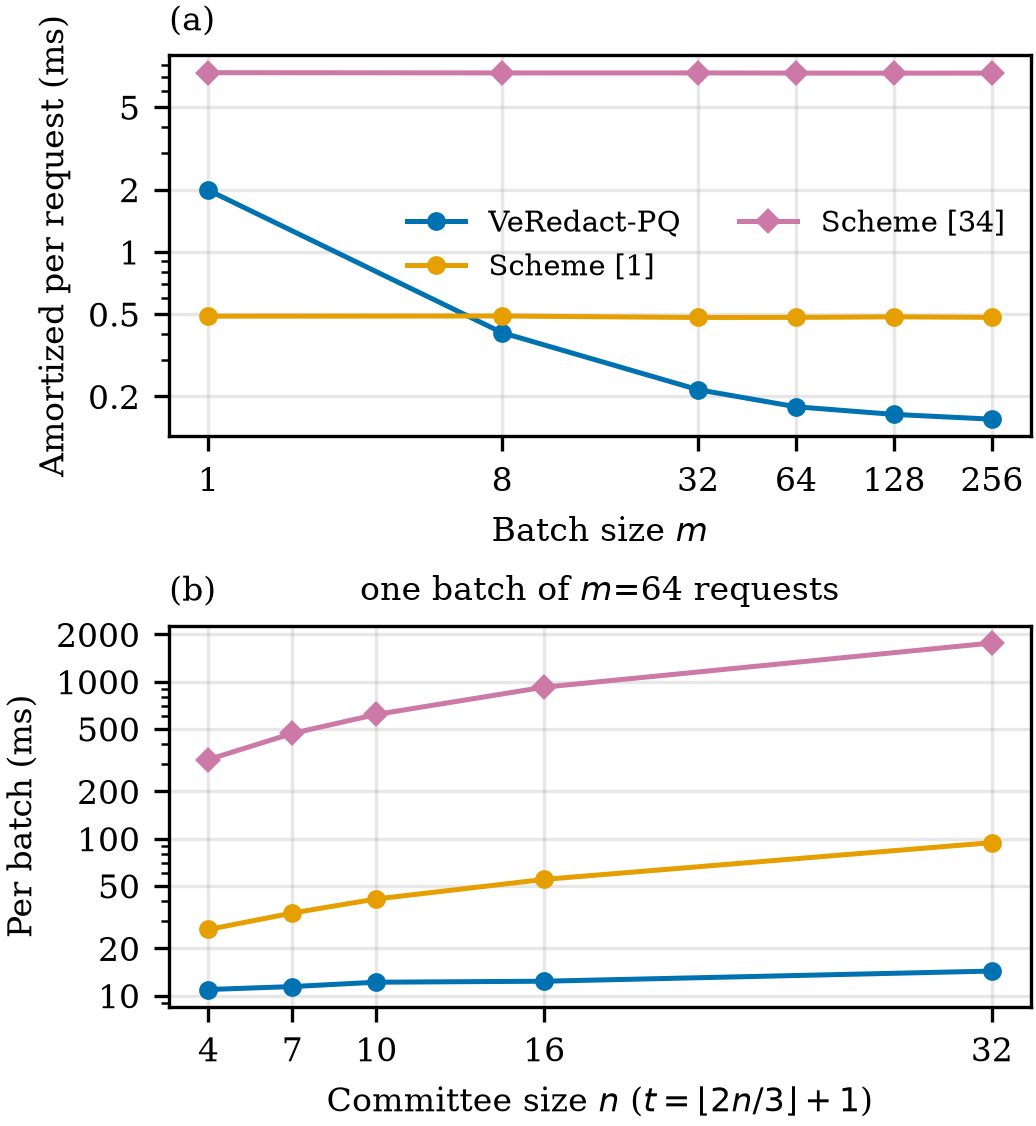
\includegraphics[width=0.8\linewidth]{exp2_authorization_latency.png}
    \caption{Authorization latency: (a) amortized latency
    per request versus batch size and (b) per-batch latency versus
    committee size.}
    \label{fig:exp2_auth}
    \end{figure}

    \chg{Fig.~\ref{fig:exp2_auth}(a) shows that the amortized authorization
    latency of VeRedact-PQ decreases from 1.99\,ms at $m=1$ to 0.41\,ms at
    $m=8$ and 0.16\,ms at $m=256$, because the $t$ committee signatures and
    their verification are shared by all $m$ requests. The baselines
    authorize every request individually, so their amortized latency
    remains constant at about 0.48\,ms for Ref.~\cite{ref1} and 7.3\,ms for
    Ref.~\cite{ref34}; VeRedact-PQ falls below Ref.~\cite{ref1} from $m=8$
    onward.}

    \chg{Fig.~\ref{fig:exp2_auth}(b) shows the latency of one batch of
    $m=64$ requests. It increases with committee size for all schemes, from
    10.9 to 14.3\,ms for VeRedact-PQ, from 26.3 to 94.2\,ms for
    Ref.~\cite{ref1}, and from 318 to 1{,}762\,ms for Ref.~\cite{ref34} as
    $n$ grows from 4 to 32. For VeRedact-PQ, this growth is incurred once per
    ABRRR batch and therefore affects all $m$ requests only through the
    amortized term $t(T_S+T_V)/m$. Consequently, larger committees, which
    strengthen distributed control, remain practical under high redaction
    volumes.}

    % ---------------------------------------------------------------------
    \subsubsection*{\textbf{Experiment 3: Audit Efficiency}}

    This experiment evaluates the service-side efficiency of Phase~6
    auditing, namely query resolution, evidence generation, and response
    size. The number of returned redaction records is varied as
    $n_Q\in\{10,10^2,10^3,10^4\}$, \chg{with records drawn from
    authorization batches of 64 requests}. VeRedact-PQ is compared with
    Scheme~\cite{ref13} and Scheme~\cite{ref1}. Response-generation
    time and response size are measured\chg{, each over 30 queries (5 for
    Scheme~\cite{ref13} at $n_Q=10^4$)}. The results are shown in
    Fig.~\ref{fig:exp3_audit}.

    \begin{figure}[t]
    \centering
    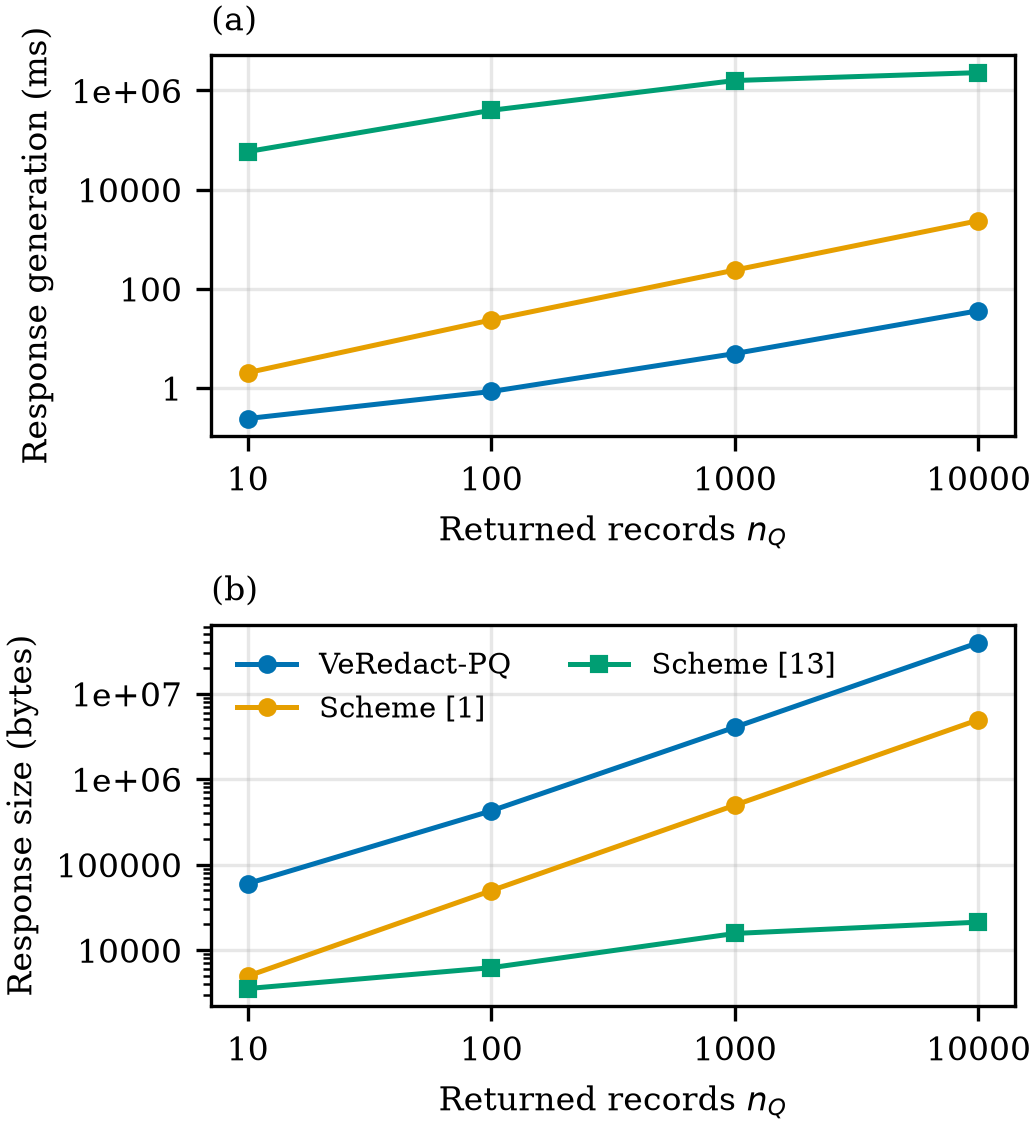
\includegraphics[width=0.8\linewidth]{exp3_audit_efficiency.png}
    \caption{Audit efficiency: (a) response-generation time
    and (b) audit-response size versus the number of returned records.}
    \label{fig:exp3_audit}
    \end{figure}

    \chg{Fig.~\ref{fig:exp3_audit}(a) shows that VeRedact-PQ generates audit
    responses fastest, from 0.24\,ms at $n_Q=10$ to 36\,ms at $n_Q=10^4$,
    because records are resolved through the sharded RAI and the
    query-scoped multiproof $MP_{Q_j}^A$ shares internal Merkle nodes.
    Ref.~\cite{ref1} requires 2.0\,ms to 2.4\,s, and Ref.~\cite{ref13}
    requires 58\,s to 38\,min, since it builds one RSA-accumulator
    non-membership witness per returned record.}

    \chg{Fig.~\ref{fig:exp3_audit}(b) shows the opposite ordering for
    response size. VeRedact-PQ returns the largest responses, from 60\,KB to
    39.6\,MB, about 4\,KB per record, dominated by the 3{,}309-byte ML-DSA-65
    validation attestation $\alpha_i$ carried by each record, whereas the
    shared authorization evidence $(R_e^{VR},C_e^B,Auth_e^B)$ is included
    only once per distinct authorization batch. Ref.~\cite{ref1} returns
    5.0\,KB to 5.0\,MB, and Ref.~\cite{ref13}, which aggregates its proof,
    returns 3.5 to 21\,KB. Overall, the results show that sharded RAI
    resolution and query-scoped evidence keep audit-service computation
    low, while post-quantum signatures dominate the communication cost of
    record-level evidence.}

    % ---------------------------------------------------------------------
    \subsubsection*{\textbf{Experiment 4: Verification Time}}

    This experiment evaluates auditor-side verification of returned
    redaction evidence. The number of verified records is varied as in
    Experiment~3 \chg{for the \textbf{Normal Audit}, which verifies validation
    attestations and the committed $H(\pi_i^{PQ})$. Verification time is
    decomposed into response signature and query binding, RAI multiproof,
    committee approvals, validation attestations, and state-transition and
    PQCH checks.} VeRedact-PQ is compared with Refs.~\cite{ref13}
    and~\cite{ref1} in their original classical instantiations. To evaluate verification granularity,
    modified, substituted, and stale evidence is additionally injected into
    \chg{1\%, 5\%, and 10\%} of returned records, and the fraction of invalid
    records individually rejected and valid records retained is measured.
    The results are shown in Fig.~\ref{fig:exp4_verify}.

    \begin{figure}[t]
    \centering
    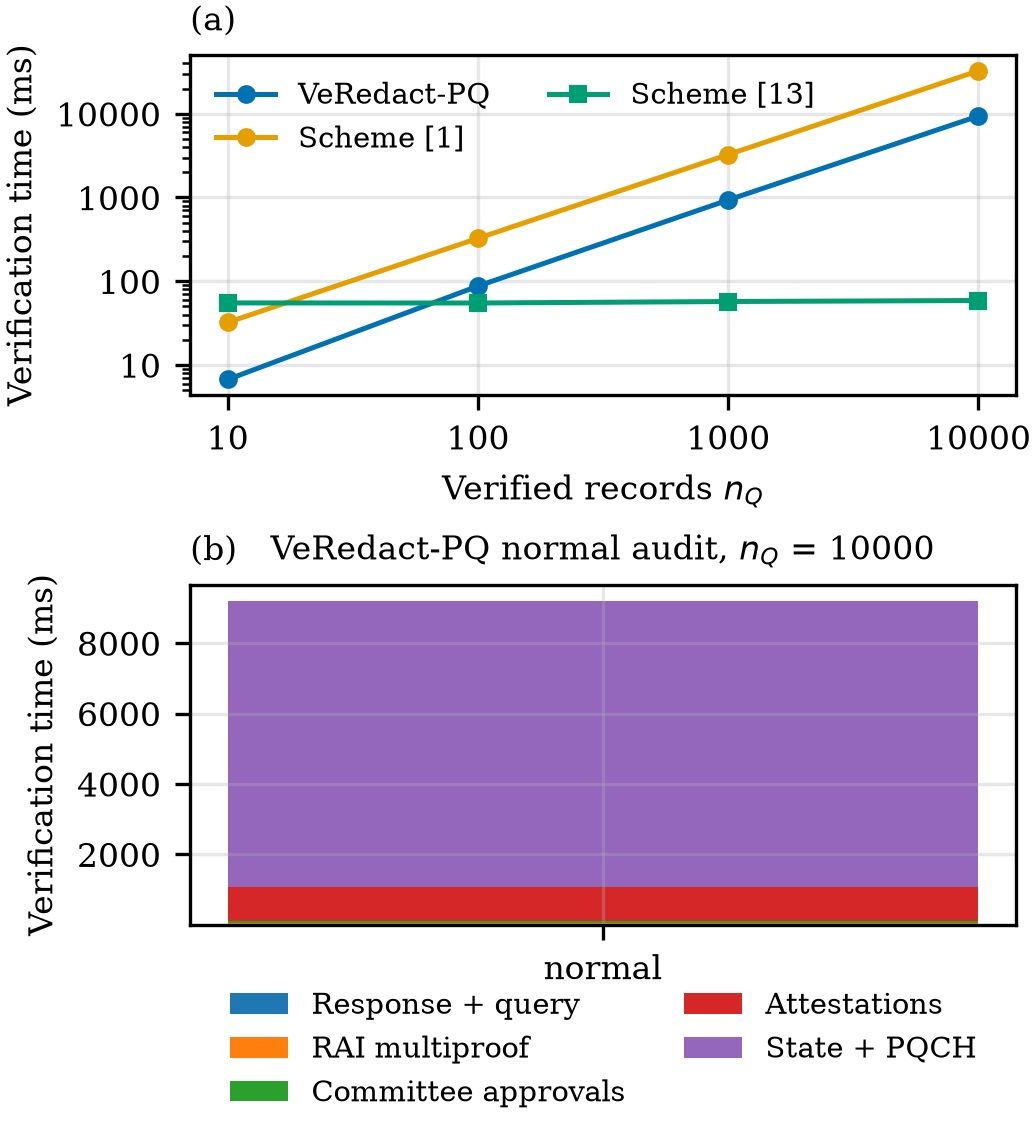
\includegraphics[width=0.8\linewidth]{exp4_verification_time.png}
    \caption{Verification time: (a) total verification time
    versus number of verified records for \chg{the normal audit} and
    (b) verification-time breakdown.}
    \label{fig:exp4_verify}
    \end{figure}

    \chg{Fig.~\ref{fig:exp4_verify}(a) shows that normal-audit verification
    time of VeRedact-PQ grows approximately linearly with $n_Q$, from
    6.7\,ms at $n_Q=10$ to 9.4\,s at $n_Q=10^4$, 3.5 to 4.8 times faster than
    Ref.~\cite{ref1} (32\,ms to 32.6\,s). Ref.~\cite{ref13} verifies one
    aggregated proof in a nearly constant 53--59\,ms and is therefore faster
    for large queries. Committee approvals contribute only
    $t|\Omega_{Q_j}^B|T_V$; routine audits therefore rely only on PQ-signed
    attestations and hash-based authentication, and complete PQZK
    verification is reserved for challenged or forensic audits.}

    \chg{Fig.~\ref{fig:exp4_verify}(b) shows the verification-time breakdown
    at $n_Q=10^4$: the state-transition and PQCH checks take 8.1\,s,
    validation attestations 0.96\,s, the RAI multiproof 57\,ms, and
    committee approvals 51\,ms. Because each returned record carries
    individual membership and execution evidence, VeRedact-PQ and
    Ref.~\cite{ref1} reject every injected modified, substituted, or stale
    record individually while retaining all valid records, as stale
    evidence fails the version, epoch, and checkpoint checks of Phase~6. In
    contrast, the aggregated decision of Ref.~\cite{ref13} rejects the whole
    response, including all valid records, whenever a single record is
    invalid.}

    % ---------------------------------------------------------------------
    \subsubsection*{\textbf{Experiment 5: Blockchain Gas Consumption}}

    This experiment evaluates the on-chain cost of VeRedact-PQ on the
    permissioned Besu network. Although the gas price is set to zero in the
    permissioned deployment, gas usage provides a deterministic measure of
    on-chain computation and storage. The measured contract operations are
    policy and committee registration (Phase~1), batch-checkpoint anchoring
    $A_b$ (Phase~2), authorization anchoring $H(Auth_e^B)$ (Phase~4), redaction finalization, which atomically commits the
    updated checkpoints $\{A_b'\}$ and SA-RLI state (Phase~5), and RAI
    checkpoint anchoring $CP_e^A$ (Phase~6). The number of redactions per
    ABRRR batch is varied as $m\in\{1,8,32,64,128,256\}$ under \chg{Zipf skew
    $s=0.8$, with 1{,}024 redactions per configuration}. The baselines were implemented as contracts that store
    the on-chain redaction state prescribed by each scheme. Total gas per
    authorization round and amortized gas per redaction are measured. The
    results are shown in Fig.~\ref{fig:exp5_gas}.

    \begin{figure}[t]
    \centering
    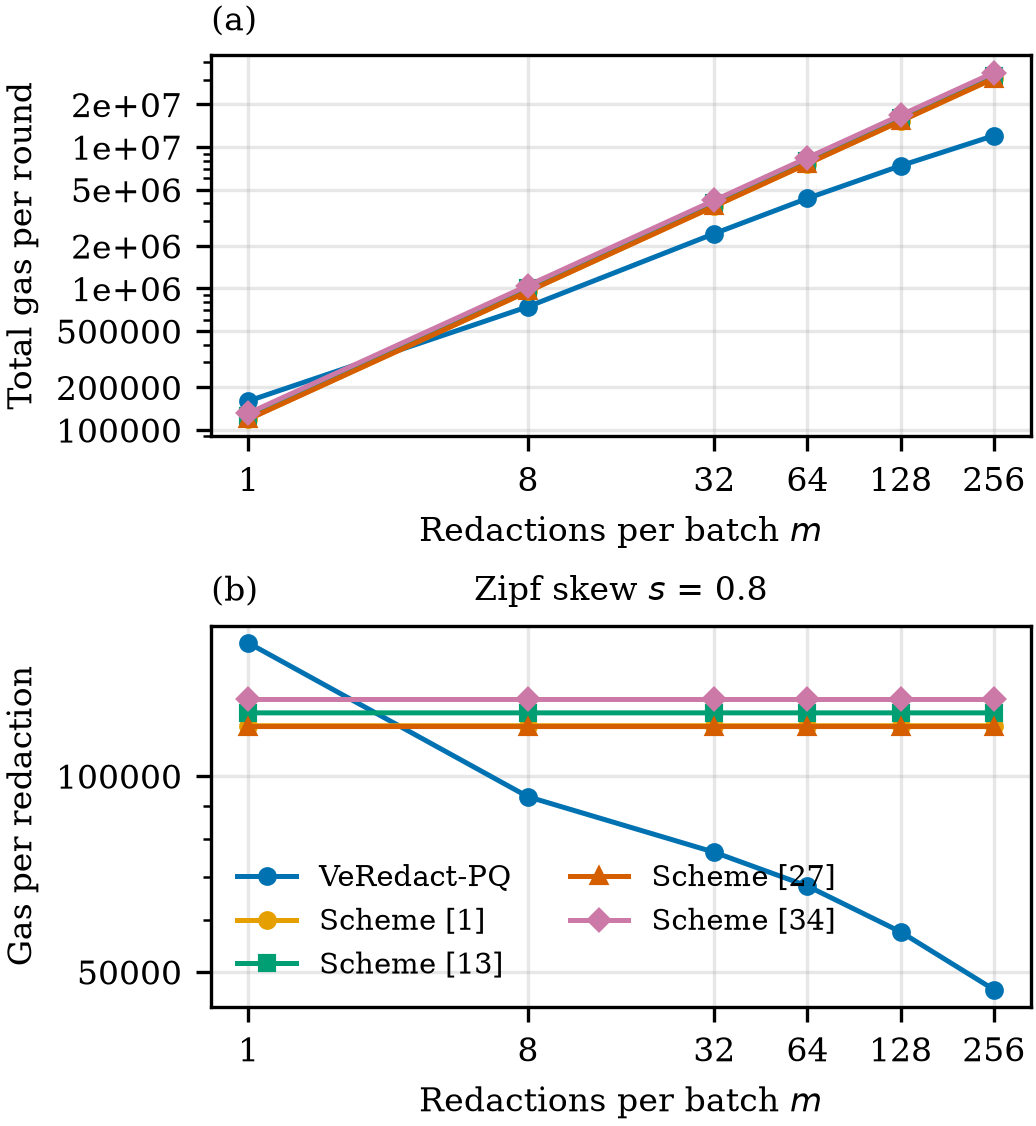
\includegraphics[width=0.8\linewidth]{exp5_gas_consumption.png}
    \caption{Gas consumption: (a) total gas per
    authorization round and (b) amortized gas per redaction versus the
    number of redactions per batch.}
    \label{fig:exp5_gas}
    \end{figure}

    \chg{Fig.~\ref{fig:exp5_gas}(a) shows that the total gas of the baselines
    increases linearly with the number of redactions because each redaction
    updates its own on-chain state, at a constant 119{,}000--131{,}000 gas
    per redaction. For VeRedact-PQ, total gas grows with the number of
    affected transaction batches $|\Omega_e|$ rather than $m$, because
    redaction finalization anchors one updated checkpoint per affected batch
    and individual redaction records are authenticated through the RAI
    checkpoint. Consequently, Fig.~\ref{fig:exp5_gas}(b) shows that the
    amortized gas per redaction decreases from 160{,}091 at $m=1$, where the
    additional authorization anchor makes VeRedact-PQ more expensive than
    the baselines, to 92{,}929 at $m=8$ and 46{,}983 at $m=256$.}

    \chg{Table~\ref{tab:gas} further reports the gas consumed by each contract
    operation. Overall, the results show that VeRedact-PQ bounds on-chain
    cost by the number of batch-root transitions and the audit-epoch
    frequency, rather than by the total redaction volume.}

    \begin{table}[t]
    \centering
    \caption{Gas Consumption of VeRedact-PQ Contract Operations}
    \label{tab:gas}
    \scriptsize
    \renewcommand{\arraystretch}{1.08}
    \setlength{\tabcolsep}{4pt}
    \begin{tabular}{lcc}
    \hline
    \textbf{Operation} & \textbf{Frequency} & \textbf{Gas} \\
    \hline
    Policy registration & Per policy version & [TBD] \\
    Committee registration & Per epoch & [TBD] \\
    Batch checkpoint $A_b$ & Per transaction batch & [TBD] \\
    Authorization anchor $H(Auth_e^B)$ & Per ABRRR batch & \chg{44{,}460} \\
    Redaction finalization $\{A_b'\}$ & Per ABRRR batch & \chg{115{,}585 ($|\Omega_e|=1$)} \\
    RAI checkpoint $CP_e^A$ & Per audit epoch & \chg{45{,}817} \\
    \hline
    \end{tabular}
    \end{table}

